\section{Internet of Things (IoT)} \label{Background-IoT}

% IoT
\npara The term \textbi{Internet of Things} or \textbi{\hyperref[Acronym-IoT]{IoT}} refers to the combination between network (internet), and physical objects (things).
It was firstly coined in 1999 by Kevin Ashton in his work of using \textit{Radio Frequency Identification} or \textit{\hyperref[Acronym-RFID]{RFID}} in a supply chain system \citep{ThatIoT}.
The \hyperref[Acronym-IoT]{IoT} devices rely on wireless communication technologies to connect them to the network.
Such technologies that allow the development of \hyperref[Acronym-IoT]{IoT} are for instance: Bluetooth, \hyperref[Acronym-RFID]{RFID}, Wi-Fi or \hyperref[Acronym-GSM]{GSM}.
As the technologies in wireless communication are continuously being developed and advanced, it allows IoT community to expand and grow significantly \citep{IoTVisionFuture}.

\subsection{Trust and Reputation System in IoT} \label{Background-IoT-Reputation}

% SIoT
\npara \textbi{Social Internet of Things} or \textbi{\hyperref[Acronym-SIoT]{SIoT}} is an integrated concept between \hyperref[Acronym-IoT]{IoT} and human social networking.
The idea is that the things in an \hyperref[Acronym-IoT]{IoT} system can discover the other devices which provide the needed services, establish a relationship and communicate with them \citep{SIoT}.
As humans do in their social life, when a person wants to know someone, or use a business service, they must know how reliable it is.
Also in the computer systems, when a device wants to use a service from the other devices, before establishing a connection with them, it should know whether the source is \textbi{trustworthy} in order to avoid problems or failures due to unexpected behaviours.

% Reputation and Trust
\npara The concept of \textbi{trust} is very subjective to each individual.
\cite{ComputationalModelTrust}'s study says that \textbi{trust} is a subjective expectation that one agent has toward another one.
It is used for expecting their future behaviours based on the encountered history.
\cite{SurveyOfTrustInComputerScience} divides the obtainment of trust in a computer system into two categories: policy-based trust and reputation-based trust.
A policy-based trust is centralised and the decision criteria are based on a third party.
The second one is based on \textbi{reputation}, which is a quantitative property derived by observed actions or behaviours in the past of one agent.
Hence, the non-centralised characteristic of the reputation-based trust allows an individual to subjectively decide its trustworthiness.

\subsection{Cloud-Fog-Edge Architecture} \label{Background-IoT-CloudFogEdge}

% Fog Introduction
\npara As the \hyperref[Acronym-IoT]{IoT} is growing and its related technologies are moving forward, an \hyperref[Acronym-IoT]{IoT} system could expand to a larger number of devices and connected sensors.
This raised consequent issues such as heavy processing and big data storage in the cloud layer or exceeding bandwidth in the network.
To tackle the problem, Cisco company proposed a solution by adding an intermediate layer between the cloud and end-device (edge) layers, called the \textbi{fog layer} \citep{CiscoUnleashFog}.

% Cloud-For-Edge
In a general \textbi{cloud-fog-edge architecture}, the \textbi{edge layer} is the most bottom layer where the end-devices are.
The devices in this layer are simplest and have less computation ability, connected to sensors or actuators in order to observe a physical phenomena or to have an interaction.
The end-devices are generally in a larger amount, and they should not perform any complex computation because they have limitations regarding hardware specification, memory and power consumption.

\npara Secondly, the \textbi{fog layer} is the intermediate layer.
The devices in this layer have more computation ability and can handle preliminary data processing as well as to store sensory data before forwarding them to the cloud layer.
In opposite direction, the fog layer can also be a middle party that passes commands or messages from the cloud layer to the edge layer.
Because the fog layer can also be geographically distributed, it can organise the edge devices in its responsible area.

\npara The last one is the \textbi{cloud layer}, which is the topmost layer in the architecture and is in charge of processing final data, managing the whole system, and storing the sensory data.
A cloud device is supposed to be physically static, and located in a data centre or a dedicated place.
The device itself can be either a dedicated server where the organisation administrator has responsibility of administration and maintenance.
Or it can be a cloud service in a form of platform-as-a-service (PaaS) or software-as-a-service (SaaS) which is provided by an external cloud service provider such as Microsoft Azure, Amazon Web Service (AWS), or Google Cloud.

%%

\section{Blockchain} \label{Background-Blockchain}

\npara \textbi{Blockchain} is a technology to store computer data in a distributed and decentralised way.
A Blockchain network is consisted of a number of \textbi{blocks}.
In a block there are \textbi{transactions} to store the data in the network.
Blocks and transactions are uniquely identified by using a cryptography hashing algorithm.
The identifier hashes of the blocks are used to link each other in a chronological linear sequence like a chain, which is the reason behind its name.

\subsection{Fundamental of Blockchain} \label{Background-Blockchain-Fundamental}

\npara \textbi{Blockchain} was originally mentioned by \cite{Bitcoin} (whose name is believed to be a pseudonym).
It proposed an electronic cash system that can store the transactions of ledgers in a decentralised way by using peer-to-peer communication.

\npara A Blockchain network has a number of blocks which are linked to each other in a chronological sequence.
As Blockchain was originally developed for storing money movements in an electronic currency called \textit{Bitcoin}, the data in each block are a set of money \textbi{transactions}.
A Blockchain node collects transactions from its clients and pack them into one block.
Then, the block is pushed to the end of the chain.
The node that has pushed the block will then broadcast the change to the other nodes in the same network to update the data.
Finally, the other nodes verify the change before updating their own chain.

\begin{figure}[htb!]
    \centering
    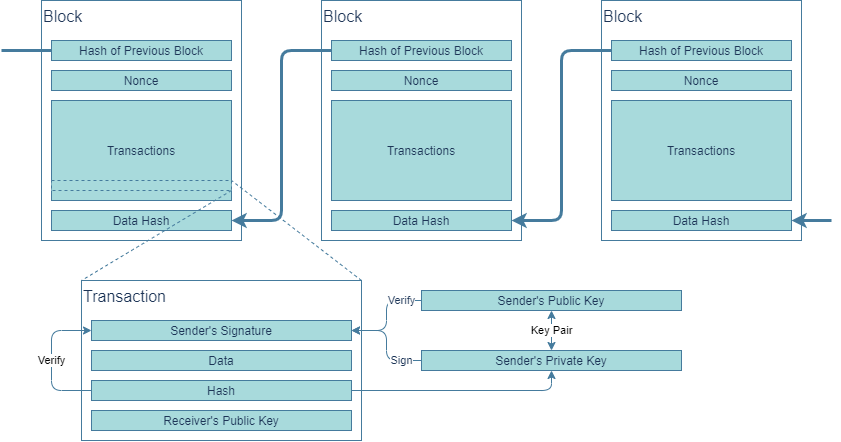
\includegraphics[width=\textwidth]{images/BackgroundBlockchain.png}
    \caption{Components of a block and transaction in a general Blockchain network}
    \label{fig:BackgroundBlockchain}
\end{figure}

\npara Figure \ref{fig:BackgroundBlockchain} shows the components inside a block.
One block contains:
  \textbi{hash of its previous block} which points to the last block in the chain before it was pushed,
  \textbi{nonce} which is a number to indicate the order of the block in the sequence,
  a set of \textbi{valid transactions},
  and the \textbi{hash} of the current block which will be referred when there is a new block afterwards.

\npara The validity of a transaction relies on the asymmetric key-pair cryptography.
A pair of \textbi{public key} and \textbi{private key} are both a set of binary data generated by mathematical techniques.
A public key can be published and generally used as an address or identifier of the owner.
In the other hand, a private key is supposed to be kept private.
It is used for signing the transaction to verify that the transaction is valid.
The public key can be generated by using a private key, but it is not possible to derive the private key from a public key.

\npara When a transaction has been generated, the creator uses its private key to sign the transaction using a mathematical calculation.
The result of the calculation is called \textbi{signature}.
The signature is then attached to the transaction before submitted to the block.
A signature can be verified whether it is valid or not by using the signer's public key.
In other words, a signature can be publicly verified by anyone but it can not be created without knowing the private key.
This is the reason why Blockchain can guarantee that the data inside will be secure and cannot be tampered even the data are visible and distributed across the network.

\npara The propagation of the data in a network becomes a problem when multiple peers want to push a new block at the same time, because the network should consider which chain from which peer node is valid and should be accepted in the chain.
This kind of problem is also known as Byzantine Generals Problem \citep{Byzantine}.
In Blockchain, the \textbi{consensus algorithm} is used to tackle the issue.
There are a number of different consensus algorithms that are used in different Blockchain implementations.
For example, Bitcoin and Ethereum uses \textbi{Proof of Work} consensus algorithm.
The Proof of Work gives a difficult mathematical challenge based on the \textit{nonce} value in the latest block.
The first node that can solve the problem has the right to push the block into the chain.
The process of calculating the mathematical problem is also called \textit{mining}.
The other examples of consensus algorithms are \textbi{Proof of Stake} which randomly select one node from the candidates using steak or wealth in the system as a random bias, or \textbi{Proof of Authority} which gives the right to an authorised node to add the block to the chain \citep{ConsensusAlgorithm}.

\subsection{Ethereum and Smart Contracts} \label{Background-Blockchain-Ethereum}

\npara \textbi{Ethereum} is a Blockchain implementation.
Similarly to Bitcoin, Ethereum blockchain also has its cryptocurrency called \textbi{Ether}.
The difference that makes Ethereum to be outstanding among developers is that Ethereum allows a block to store executable programmes.
This kind of applications is called \textbi{Smart Contract}.
A Smart Contract allows the execution and the storage of the programme stage to be done in a distributed and decentralised way.
The operation codes (opcode) in the Smart Contract were designed to be \textit{Turing complete}, which means that it can execute any programme algorithms that the actual computers can perform \citep{EthereumWhite}.

\npara Similar to the other Blockchain implementations, all nodes in Ethereum network contains the same transactions data, including Smart Contracts and their contract states.
This concept is like having a computer whose instances are distributed over the Blockchain network.
When a contract method is called, the node will add the method calling transaction into the chain.
The transaction can be interpreted and executed to update the contract state.
When the transaction is propagated over the network, the other nodes will also update their contract state in the same way.
This distributed machine is called \textbi{Ethereum Virtual Machine (\hyperref[Acronym-EVM]{EVM})}.

\begin{figure}[htb!]
  \centering
  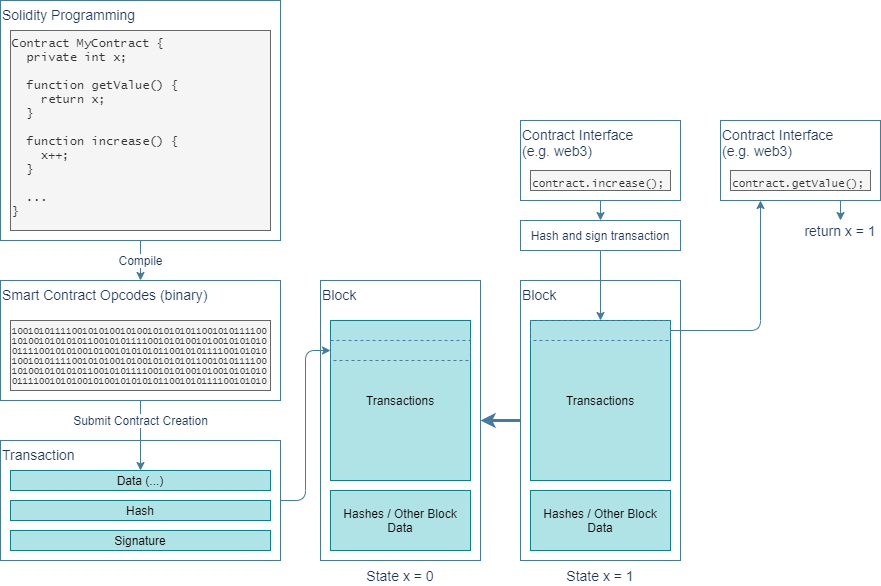
\includegraphics[width=\textwidth]{images/BackgroundEthereum.png}
  \caption{An example flow of contract creation and function calling in Ethereum Smart Contract}
  \label{fig:BackgroundEthereum}
\end{figure}

\npara Figure \ref{fig:BackgroundEthereum} shows the workflow of an Ethereum Smart Contract.
The top level programming language to write a Smart Contract can be either \textbi{Solidity} or \textbi{Vyper}, which has the similar syntax to JavaScript and Python respectively.
After that, the programming codes are compiled into Ethereum opcode binaries.
An opcode indicates a computational operation of the \hyperref[Acronym-EVM]{EVM} like an opcode in a computer programme.
These binaries data are then embedded into a transaction in a block and pushed into the chain.
The figure \ref{fig:BackgroundEthereum} also shows that calling method which changes the contract state (altering the variable value in the contract) needs to be submitted as another transaction in another block.
However, if the method is read-only (returns the contract state value without updating it), it can be called instantly without submitting as another transaction.

Calling a method in the Smart Contracts needs to be payed by its cryptocurrency.
The price of a method calling is determined by \textit{gas} spent in the calculation.
The concept of \textit{gas} is similar to the electric consumption in a physical computer.
Each opcode in a Smart Contract spends a different amount of gas determined by Ethereum\footnote{Ethereum gas per opcode: \hyperlink{https://docs.google.com/spreadsheets/d/1m89CVujrQe5LAFJ8-YAUCcNK950dUzMQPMJBxRtGCqs}{\code{https://docs.google.com/spreadsheets/d/\newline
1m89CVujrQe5LAFJ8-YAUCcNK950dUzMQPMJBxRtGCqs}}}.
The maximum amount of gas is limited by the Ethereum network.
For this reason, a method which has too many operations, especially iterations, is likely to cause an \textit{out of gas} error from the Ethereum network.

\npara

%%

\section{Spatial Indexing} \label{Background-SpatialIndexing}

\npara A computer processes and handles data in binary.
Therefore, the data that are not based on binary integer require more complicated data structures and different standards to work with, for instance, decimal (floating) number, text, picture, sound, as well as geospatial data.
Querying and accessing these types of data can be improved in performance and efficiency by using \textbi{indexing techniques}.
Indexing technique constructs the desired data to be a certain kind of search-able keywords.
When a user wants to query for the data, it can use a lookup table containing the sorted indices to quickly look for the position where the desired data are located.

\npara However, indexing the geographical data is more complicated as it is multidimensional and generally related to Euclidean space \citep{SpatialIndexing}.
There are different ways to index the geospatial data, for example, R-Tree which is based on a binary search tree for range query of destination spatial object \citep{RTrees}.
This thesis will focus on the geocoding-based indexing techniques to store and query for the spatial data objects in the Blockchain.

\npara \textbi{Geocoding} is the conversion of a geospatial object into another kind of interpretation.
Some geocoding techniques aim to ease human readability, postal address for example.
In the other hand, some of them aim to ease the readability and indexing in machine as the geocoded value is resulted in a binary integer, such as \textbi{Geohash} and \textbi{S2}, which are going to be studied in this thesis.
However, geocoding techniques are not two-way compatible.
In other words, the geocoded information cannot be reverted to the exact same geospatial object, but only to a similar one \citep{FastGeohash}.
Nevertheless, loss of accuracy is tolerable in this work, as its aim is not to store the exact geospatial data, but is to use them as an additional contextual information of the reputation management in an \hyperref[Acronym-IoT]{IoT} system.

\subsection{Geohash}

\npara \textbi{Geohash} is a hierarchical geocoding technique.
As it is hierarchical, Geohash representation does not have a fixed length, but the longer it is, the more precise geographical location it can describe.
A Geohash defines a location by storing binary bits of longitude in the odd positions, and latitude in the even positions (when the first position starts with 1).
However, it is more common to represent this group of binary bits into a textual representation, by grouping them into five bits per group and use \textbi{base32 representation} to textualise the data \citep{GeohashIndex}.
(Appendix \textit{\nameref{Appendix-Base32}})

\begin{figure}[htb!]
  \centering
  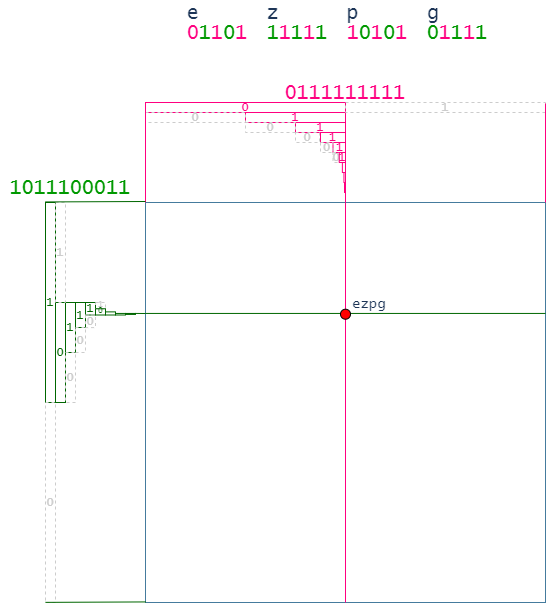
\includegraphics[width=\textwidth]{images/BackgroundGeohash.png}
  \caption{Example of the interpretation of a Geohash string into the geographical object}
  \label{fig:BackgroundGeohash}
\end{figure}

\npara Figure \ref{fig:BackgroundGeohash} shows an example of how Geohash works.
The figure gives an example of Geohash string \code{ezpg}.
The alphabets are base32-encoded character which can be converted to binary: \code{e} is \code{01101}, \code{z} is \code{11111}, \code{p} is \code{10101}, and \code{g} is \code{01111}.
Then, these binaries are concatenated.
Those bits at the odd positions (pink in Figure \ref{fig:BackgroundGeohash}) represent the longitude or x axis, and those at the even positions (green in Figure \ref{fig:BackgroundGeohash}) represent the latitude or y axis.
In the longitudinal bits, \code{0} represents the left side and \code{1} represents the right side.
But when the interpretation is on the geometric earth, it will start by taking the longitude 0° as the middle point.
When the bit is \code{0} it will travel to the minus side of the middle point (-180° to 0°), while in the case of \code{1} it will travel to the plus side of the middle point (0° to 180°).
For the next bit position, the new middle point will be calculated, and takes the same step over and over until the end of the sequence.
Similarly for the latitudinal bits, \code{0} represents the lower side from the middle point and \code{1} represents the upper side, when the first middle point is the equator.

\npara The Geohash then preserves the hierarchical property, as when it is represented by a less number of bits, the area (or the error) will be larger and is more difficult to define a point in the area.
But the more bits it gains, the smaller the area shrinks.
For this reason, two Geohashes having a mutual prefix means that they are located in the same cell at the upper level.

\subsection{S2}

\npara \textbi{S2} is another hierarchical geocoding technique similar to Geohash.
It is represented by an integer with a maximum of 64 bits in length.
Because it is hierarchical, like Geohash, the length of the representation can be reduced, but there will be a loss of its accuracy as the represented area will be bigger \citep{GeofencesBlockchain}.

\begin{figure}[htb!]
    \centering
    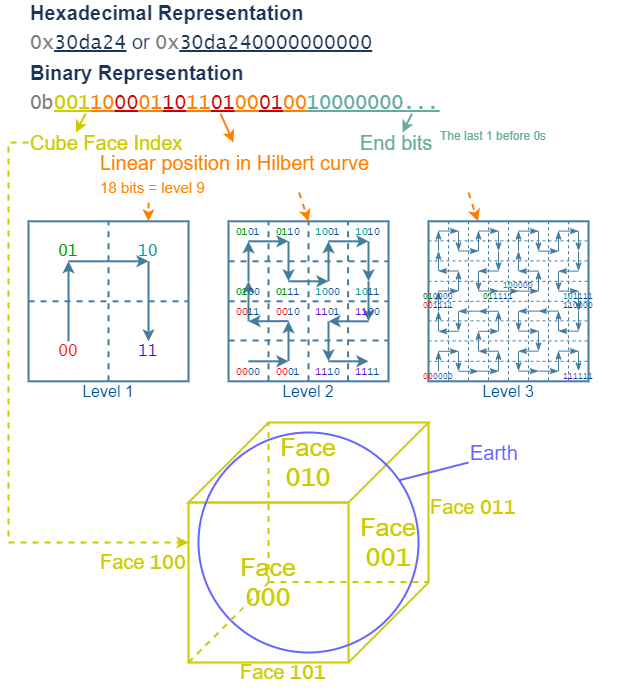
\includegraphics[width=\textwidth]{images/BackgroundS2.png}
    \caption{Example of interpretation of S2 cells}
    \label{fig:BackgroundS2}
\end{figure}

\npara One difference between Geohash and S2 is that S2 cells are based on the Hilbert space-filling curve, which is a line that travels through all the cells in a tabular space without making any loops.

\npara Figure \ref{fig:BackgroundS2} shows the characteristics and the interpretation of S2.
The length of an S2 representation can be 64 bits in maximum, but it can be trimmed to the desired level to reduce space consumption.
The end of S2 is determined by the last bit \code{1} that is followed by \code{0}s until the end of the data length.
Those bits before that are significant for calculation and cannot be cut, otherwise, the precision will be lost.
An area represented in S2 is called \textbi{cell}, which is the term that will be used in this thesis to refer a geocoded area in either Geohash or S2.

\npara As S2 uses a cube to fit the earth sphere and project the location to each face of the cube, the first 3 bits of an S2 cell are preserved for determining in which face the cell is falling in\footnote{\url{https://s2geometry.io/resources/earthcube}} (from \code{000} for the first face, until \code{101} for the sixth face).
The next set of the binary data represents the linear position on the Hilbert curve.
One cell position in the Hilbert curve contains 4 cells in the next level.
Hence, every level increment requires 2 more bits.

\npara The example in Figure \ref{fig:BackgroundS2} shows that \code{100001101101000100} contains 18 bits, which means the cell is located in 138,053\textsuperscript{rd} region in level-9 of the Hilbert curve, out of all 262,144 regions (which is 4\textsuperscript{9}).
The figure also demonstrates that, decreasing level of the Hilbert curve, the cell still covers the same region but in a bigger area.
This also implies that when two cells have a mutual prefix, they are located in the same cell of the upper level, which is the same property that Geohash also has.
